\documentclass[11pt]{article}
\usepackage{geometry}                % See geometry.pdf to learn the layout options. There are lots.
\geometry{letterpaper}                   % ... or a4paper or a5paper or ... 
%\geometry{landscape}                % Activate for for rotated page geometry
%\usepackage[parfill]{parskip}    % Activate to begin paragraphs with an empty line rather than an indent
\usepackage{graphicx}
\usepackage{amssymb}
\usepackage{epstopdf}
\usepackage{ulem}
\usepackage{url}

\usepackage{wrapfig}
\usepackage{subfig}

\textwidth 6in
\textheight 9in

\graphicspath{{images/}}

\DeclareGraphicsRule{.tif}{png}{.png}{`convert #1 `dirname #1`/`basename #1 .tif`.png}

%\title{Flying \xout{On} Empty}
\title{Delayed, Cancelled, On Time, Boarding ... Flying over the USA}
\author{Statistical Graphics Working Group, Iowa State University}
\date{\today}                                           % Activate to display a given date or no date

\begin{document}
%\maketitle
%\tableofcontents
%\begin{abstract}
%\end{abstract}
\section{Contribution of ISU's working group `Statistical Graphics'}
%\subsection*{Heike Hofmann, Dianne Cook, Christopher Kilion, Barret Schloerke}
\subsection{Flight Volume \& Delays}
Flight volumes overall is on the increase (see figure\ref{volume} for four major airports).  Structural shifts in the loads of airports led to minimal average delays in `02 and `03 (see figure \ref{delays}). Average delays have been increasing since. Delays build up during the day, with a maximum reached in the early evening hours. 
\begin{figure}[htbp] %  figure placement: here, top, bottom, or page
   \centering
   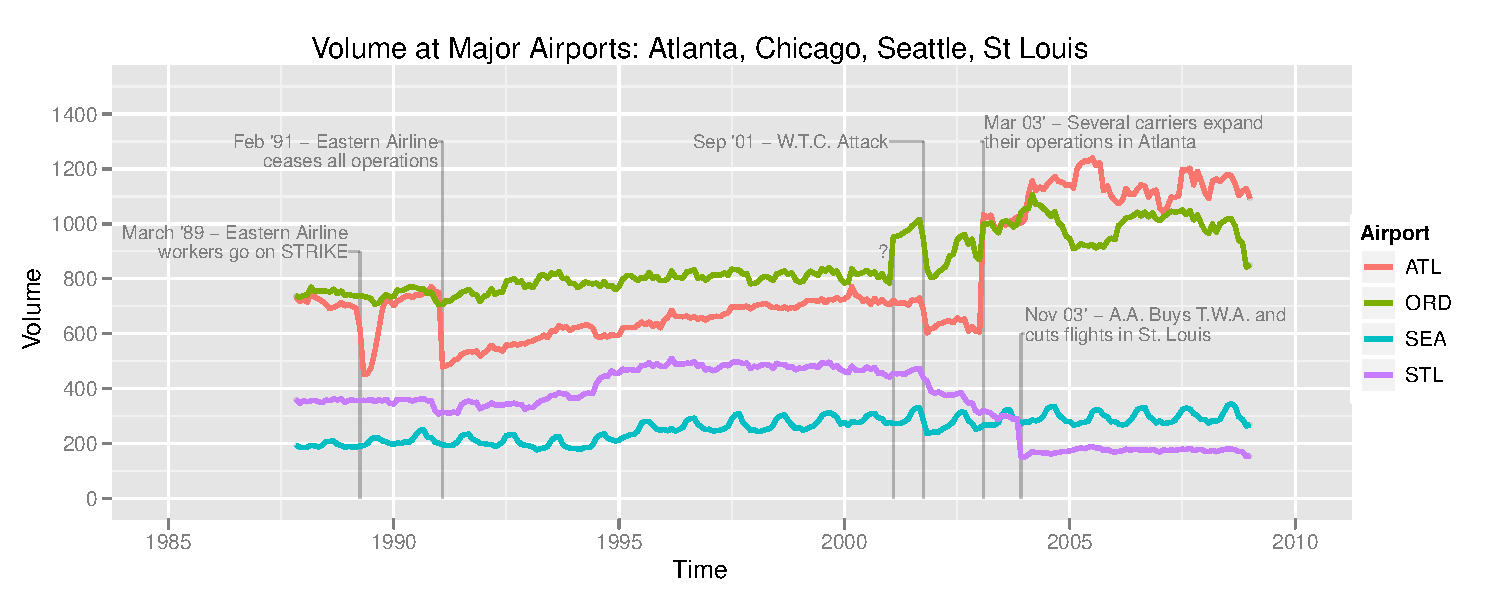
\includegraphics[width=4.5in]{airports.pdf} 
   \caption{Flight volumes at four major airports shown as daily number of flights over time. Atlanta (ATL) shows the largest structural changes during the time period. Seattle-Tacoma (SEA) exhibits a strong seasonal pattern.}
   \label{volume}
\end{figure}

\begin{figure}[htbp] %  figure placement: here, top, bottom, or page
   \centering
   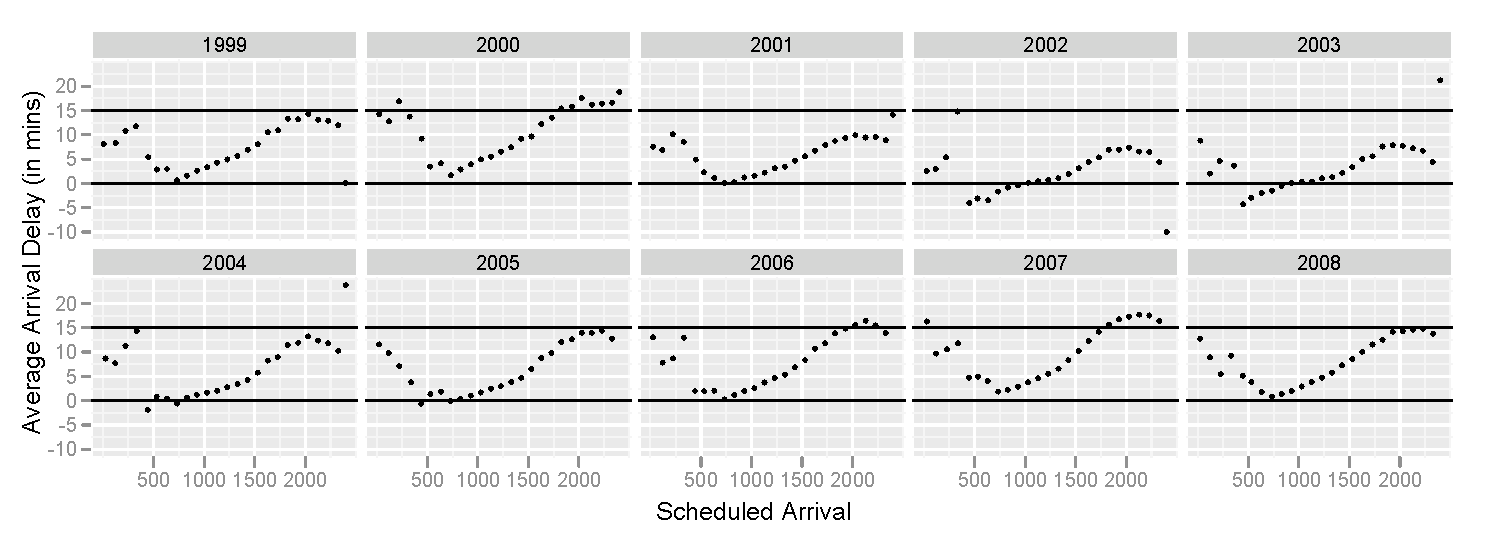
\includegraphics[width=5in]{arrdelay-crsarrtime.pdf} 
   \caption{Average arrival delays over the course of a day. Delays build up quite considerably throughout the day. During 2001 -- 2003 delays were  cut back from previous years, but have crept back up again.}
   \label{delays}
\end{figure}


\subsection{Ghosts of Flights}
%One interesting aspect of the data is, however, what can not be found in this database: when planes fly empty between airports. This problem is - to different degrees - common across all airline carriers, e.g.
%In 2007 British Airways was criticized heavily in the media for flying empty planes, so called ``ghost planes", across the Atlantic, 
%%(see http://www.cbc.ca/world/story/2007/11/13/ba-flights.html?ref=rss)
%which  clashed with the environmentally friendly image the company was promoting at the time. 
%
%Enplanement information  is not publicly available,  making checks for empty planes impossible. However, 
Tail numbers uniquely identify a plane and are recorded electronically during take-off and landing making it possible to track each aircraft's journey over its lifetime. Flight paths re-constructed form the data show interruptions, that is, a plane takes off from a different location than it last landed. We have to assume that the plane covered  (at least) this distance in the air - and -- with the exception of international flights -- was flying empty as a {\it ghost flight}.

%Table \ref{march-8} shows an excerpt of the flight path of machine N881US, a two-engine Fokker with 111 seats, for March 8, 1995. Flight 557 from Covington, KY, is diverted to Pittsburgh, PA, resulting in a 222 mile long ``ghost flight" from Pittsburgh to Richmond, VA. 
%
%%%Obviously, ghost flights can happen for various reasons: flights get cancelled, planes are diverted, planes might need maintenance not available at the local airport, additional planes might be needed during adverse weather events, or flight schedules might require a plane to be at a specific airport. 
%
%%%\subsubsection{Example: Aircraft N881US}
%%Probably all of these are reasons for the 110 ``ghosts" produced by the aircraft N881US, a two-engine Fokker with 111 seats, which was put into service by United Airways on Jan 1 1995, last flown on Dec 19th 2000, and exported to the Netherlands in 2003. 
%%% i found different information on http://www.airframes.org/reg/n881us
%%% i got the previous information from Chris' database
%%The Data Expo '09 registers 14082 flights of this aircraft, which makes a ``ghost rate" of less than 1\%.
%%% miles flown empty percentage?
%%% can we be sure that this machine did not make international trips?
%
%%Table \ref{march-8} shows an excerpt of the flight path of machine N881US for march 8, 1995. Flight 557 from Covington, KY, is diverted to Pittsburgh, PA, resulting in a 222 mile long ``ghost flight" from Pittsburgh to Richmond, VA. 
%
%\begin{table}[htb]
%\centering
%\vspace{-5pt}
%\begin{tabular}{rrccr} \hline
%\bf Departure & \bf Arrival & \bf Origin & \bf Dest & \bf Diverted \\ \hline\hline
%11:02 & 12:56 & PIT & CVG &     0\\
%13:11 &   NA & CVG & PIT &     1\\
%19:13 & 20:50 & RIC & PIT     & 0\\
%21:34 & 23:00 & PIT & MSY &     0\\\hline
%\end{tabular}
%\vspace{-10pt}
%\caption{\it \label{march-8} Flight path of aircraft N881US on March 8 1995.}
%\vspace{-10pt}
%\end{table}

%On the evening of April 28, 95 the aircraft lands at Kalamazoo, MI,  and takes off in the morning of the 29th from Pittsburgh (presumably having overnight flown the 301 miles distance between the airports without passengers). Table \ref{april} shows this part of the flight path of aircraft N881US.

%\begin{table}[htb]
%\begin{center}
%{\tt \begin{verbatim}
%    Year Month DayofMonth DepTime ArrTime Origin Dest
%582 1995     4         28    1815    1936    GSO  PIT    
%684 1995     4         28    2024    2133    PIT  AZO     
%613 1995     4         29     823     935    PIT  RDU     
%597 1995     4         29    1011    1124    RDU  PIT   
%\end{verbatim}}
%\caption{\it \label{april} Flight path of aircraft N881US on the evening of April 28th and morning of April 29th 1995.}
%\end{center}
%\end{table}

%%Figure \ref{map-n881us} shows an overview of all the flights of aircraft N881US. Sites of airports are drawn as points on a map, the point size is determined by the number of flights into each airport. Lines are drawn for flights between airports, the width of the lines is proportional to the number of times the route was flown. 

%%\begin{figure}[htbp] %  figure placement: here, top, bottom, or page
%%   \centering
%%   \includegraphics[width=6in]{images/map-n881us.pdf} 
%%   \caption{\it Track of all the flights of aircraft N881US during its lifetime at US Airways. Size of points and widths of lines correspond to number of flights into an airport and number of flights between locations, respectively. Major airports for this plane are Charlotte, SC, and Pittsburgh, PA, as well as some airports in the Metro-Area between DC and Boston along the East Coast.}
%%   \label{map-n881us}
%%   % poduced by flight-path.R
%%\end{figure}
%%% some resultsOO, 
%%% outline of the paper

%This same procedure of calculating ghost flights is repeated for every aircraft individually and then gathered for every airline.
%For the period of 1995 - 2008, this results in over 1 million flights, flying a minimal average distance of 1000 miles. Since 2001 air carriers have been cutting down on the number of ghost flights, particularly major airlines. Smaller carriers are facing increasing costs from ghosts flights (due to increases in fuel costs). 
Figure \ref{ghosts} shows all ghost flights for Hawaiian Airline (HA), Jetblue Airways (B6) and Airtran Airways Corporation (FL) in 2008. Neither one of these carriers did fly internationally during that time. 


\begin{figure}[hbtp]
\vspace{-10pt}
  \centering
  \subfloat[Hawaiian Airlines (HA)]{\label{ghost:hal}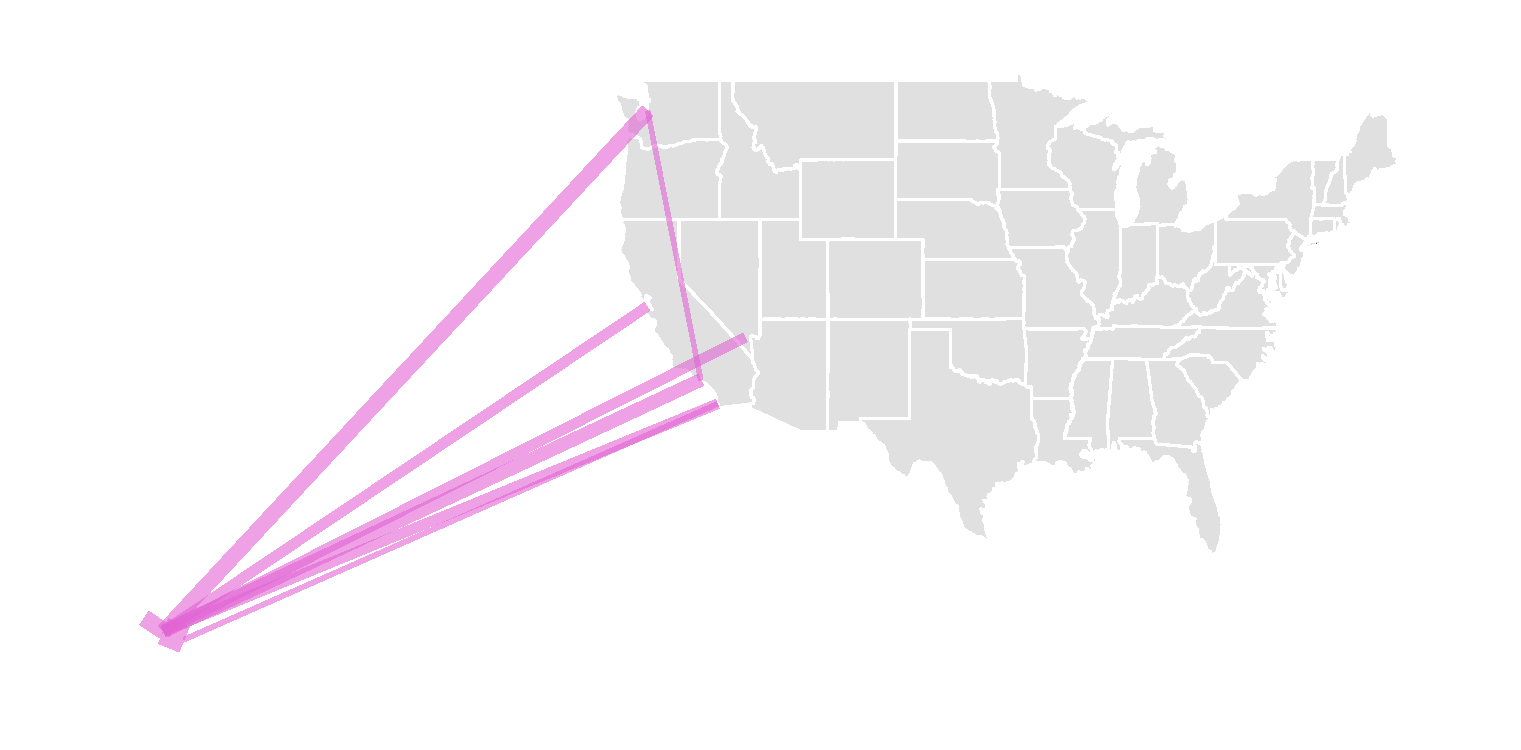
\includegraphics[height=1.15in]{map-ha-08}}    
  \hfill             
 \hspace{-5pt}  \subfloat[Airtran Airways Corporation (FL)]{\label{ghost:fl}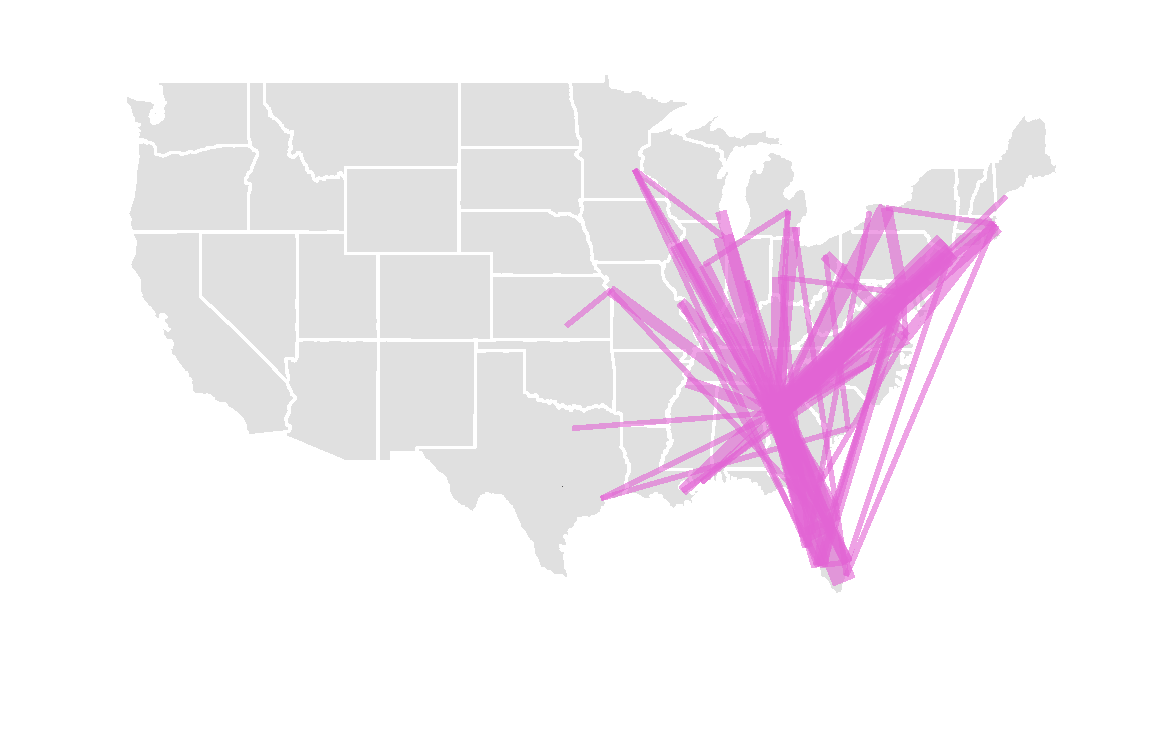
\includegraphics[height=1.0in]{map-fl-08}}
 \hfill
  \subfloat[Jetblue Airways (B6)]{\label{ghost:b6}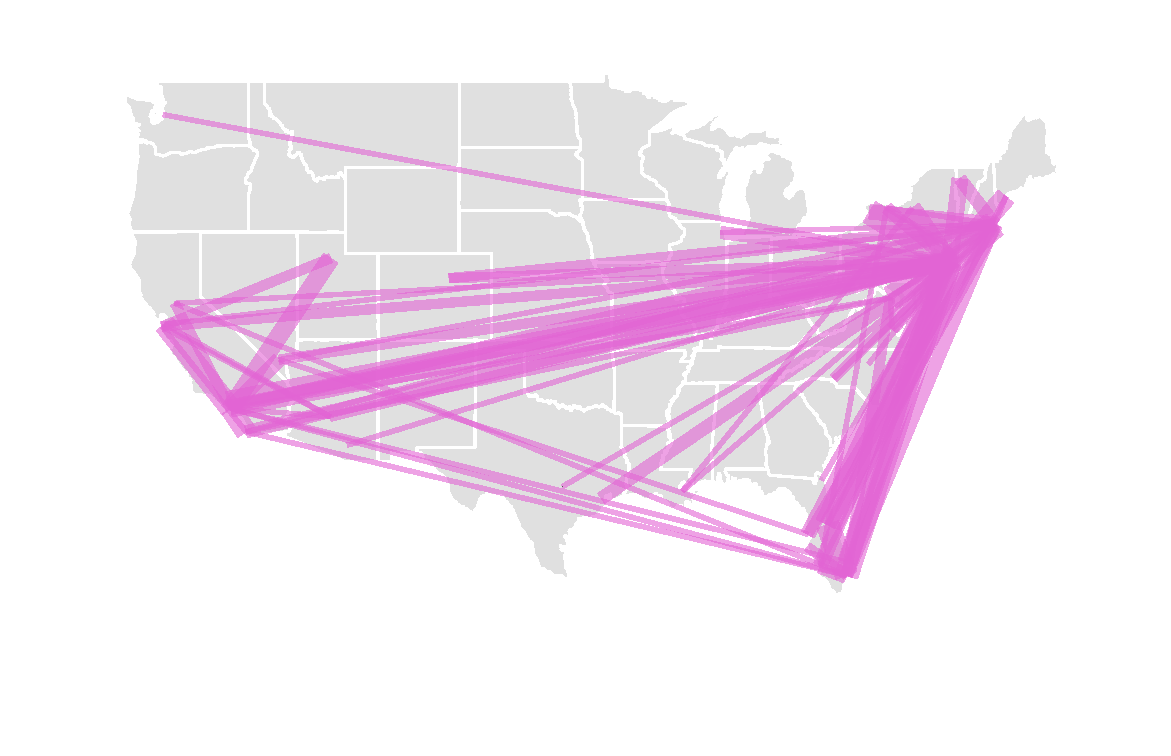
\includegraphics[height=1.0in]{map-b6-08}}
\vspace{-10pt}
  \caption{\it Ghosts flights of three local carriers in 2008.}
  \label{ghosts}
\end{figure}

%\subsection{Fuel Costs and Consumption}
%% more results of ghost flights per airline carrier
%Besides being interesting in themselves (or so we would like to think), ghost flights might also be used in assessing how cost effective and ``green" an airline is run.
%Since 2000 airline carriers are required to provide monthly reports on fuel consumption for both scheduled and unscheduled flights and can be downloaded from the Bureau of Transportation Statistics website at http://www.transtats.bts.gov/.  
%Complete data, particularly for the portion of fuel for unscheduled flights, is available only for major airlines. Fuel consumption for unscheduled flights should, at least partly, come from ghost flights. 

%% summary of fuel for unscheduled flights
%Fuel consumption reported by airlines for unscheduled flights appears to be largely unrelated to overall miles flown or the size of the airline carrier. Figure \ref{fuel-unscheduled} gives an overview of the percentage of fuel reported by airline carriers for unscheduled purposes compared to overall fuel consumption. The highest percentage is close to 20\% for carrier TZ - that is ATA Airlines, who ceased operations in April 2008. Some carriers report no expenditure for unscheduled flights, among them: B6, FL, MQ, and YV. Some companies have recently started to report non-zero fuel consumption for unscheduled domestic travel, such as WN and XE. AQ seems to have reported a fixed 0.5\% of total fuel consumption for unscheduled flight for some years, but recently switched to report 0. Besides Hawaiian airlines and OH, most airlines report fuel consumptions for unscheduled flights as below  1\% of all total fuel costs.

%\begin{figure}[htbp] %  figure placement: here, top, bottom, or page
%   \centering
%   \includegraphics[width=6in]{images/fuel-unscheduled.pdf} 
%   \caption{\it Time series of percentage fuel consumption for unscheduled flights compared to overall fuel consumption. }
%   \label{fuel-unscheduled}
%   % poduced by fuel-miles.R
%\end{figure}

%Figure \ref{fuel-miles} shows a set of scatterplots of miles flown (in millions) versus fuel consumption (in million of gallons) for the years 2000 to 2008. A linear relationship between fuel consumption and distance covered would be expected. Remember, that these data come from different sources: fuel consumption is reported by airline carriers, whereas distance flown is derived from the data recorded on each commercial flight. The overall linear relationship of the data is therefore re-assuring. 
%Interestingly, the exact nature of the relationship between miles flown and fuel consumption does not seem to be the same for all airline carriers.  Some airline carriers appear to need a lot more fuel for the same distance. Some structural changes also become apparent over time: initially, three big airline carriers (American Airlines, Delta and United Airlines) were in the lead, with four medium-sized airline carriers following (Continental, Northwest, Southwest and US Airways). In 2008, the picture has changed: American Airlines and Southwest are now the big players, with the other airlines in pursuit.

%\begin{figure}[htbp] %  figure placement: here, top, bottom, or page
%   \centering
%   \includegraphics[width=6in]{images/fuel-miles.pdf} 
%   \caption{\it Scatterplots of Fuel consumption (in millions of gallons) versus Miles flown (in millions). Airline carriers are color-coded. A strong linear relationship becomes obvious. Interestingly, not all carriers seem to have the same slope. }
%   \label{fuel-miles}
%   % poduced by fuel-miles.R
%\end{figure}

%Figure \ref{fuel-2007} shows a dotplot of the average fuel consumption of an airliner carrier for the year 2007. We can use this plot for a visual assessment of how fuel-effective different airlines are managed. From left to right effectiveness declines. Small carriers, such as SkyWest (OO), XE, MQ, and YV have the least fuel needs on 100 million miles, whereas big airline carriers such as DL,  AA, NW have higher fuel consumption on 100 million miles. Hawaiian Airlines comes in at just under 400 Million Gallons fuel consumption on 100 million miles flown, almost fourfold the fuel consumption than SkyWest. 

%\begin{figure}[htbp] %  figure placement: here, top, bottom, or page
%   \centering
%   \includegraphics[width=6in]{images/fuel-2007.pdf} 
%   \caption{\it Dotplot of average fuel consumption for each airline carrier on 100 million miles in 2007. The range in fuel consumption is between just under 100 Mio Gallons to close to 400 Mio Gallons. }
%   \label{fuel-2007}
%   % poduced by fuel-miles.R
%\end{figure}

%Figure \ref{ha-ghosts} shows an image produced by Google Earth of all ghost flights made by Hawaiian Airlines in 2006.

%\begin{figure}[htbp] %  figure placement: here, top, bottom, or page
%   \centering
%   \includegraphics[width=4in]{images/ha-ghosts.pdf} 
%   \caption{\it  Tracks of ghost flights by (HA) Hawaiian Airlines in 2006. Thickness of lines corresponds to number of flights made between connected airports. }
%   \label{ha-ghosts}
%   % poduced by fuel-miles.R
%\end{figure}



\subsection{Windy Situations}
%Every airport has a weather station associated with it. This data is available to at least an hourly resolution from websites such as Weather Underground (www.wunderground.com) for almost all airports across the US covering several years of data. Based on this, we can link information of weather situations to scheduled flight take-off and landing times in order to explore the existence and strength of the weather's effect on delays.
%Obvious results include delays corresponding to weather situations causing reductions in sight, such as fog, rain and snowfall - in Chicago O'Hare each inch of snow accumulation corresponds to an average expected delay of 15 minutes. 
Do crosswinds have an impact on on-time performance? - We tried to answer this question at the example of Phoenix International Airport, where all three runways are oriented West-East (see figure \ref{phx}). Weather data collected at Phoenix Skyharbor (PHX) published  by Weather Underground (\url{http://www.wunderground.com}) is linked to the Expo Data. 

\begin{wrapfigure}{r}{0.35\textwidth}
\vspace{-25pt}
  \begin{center}
    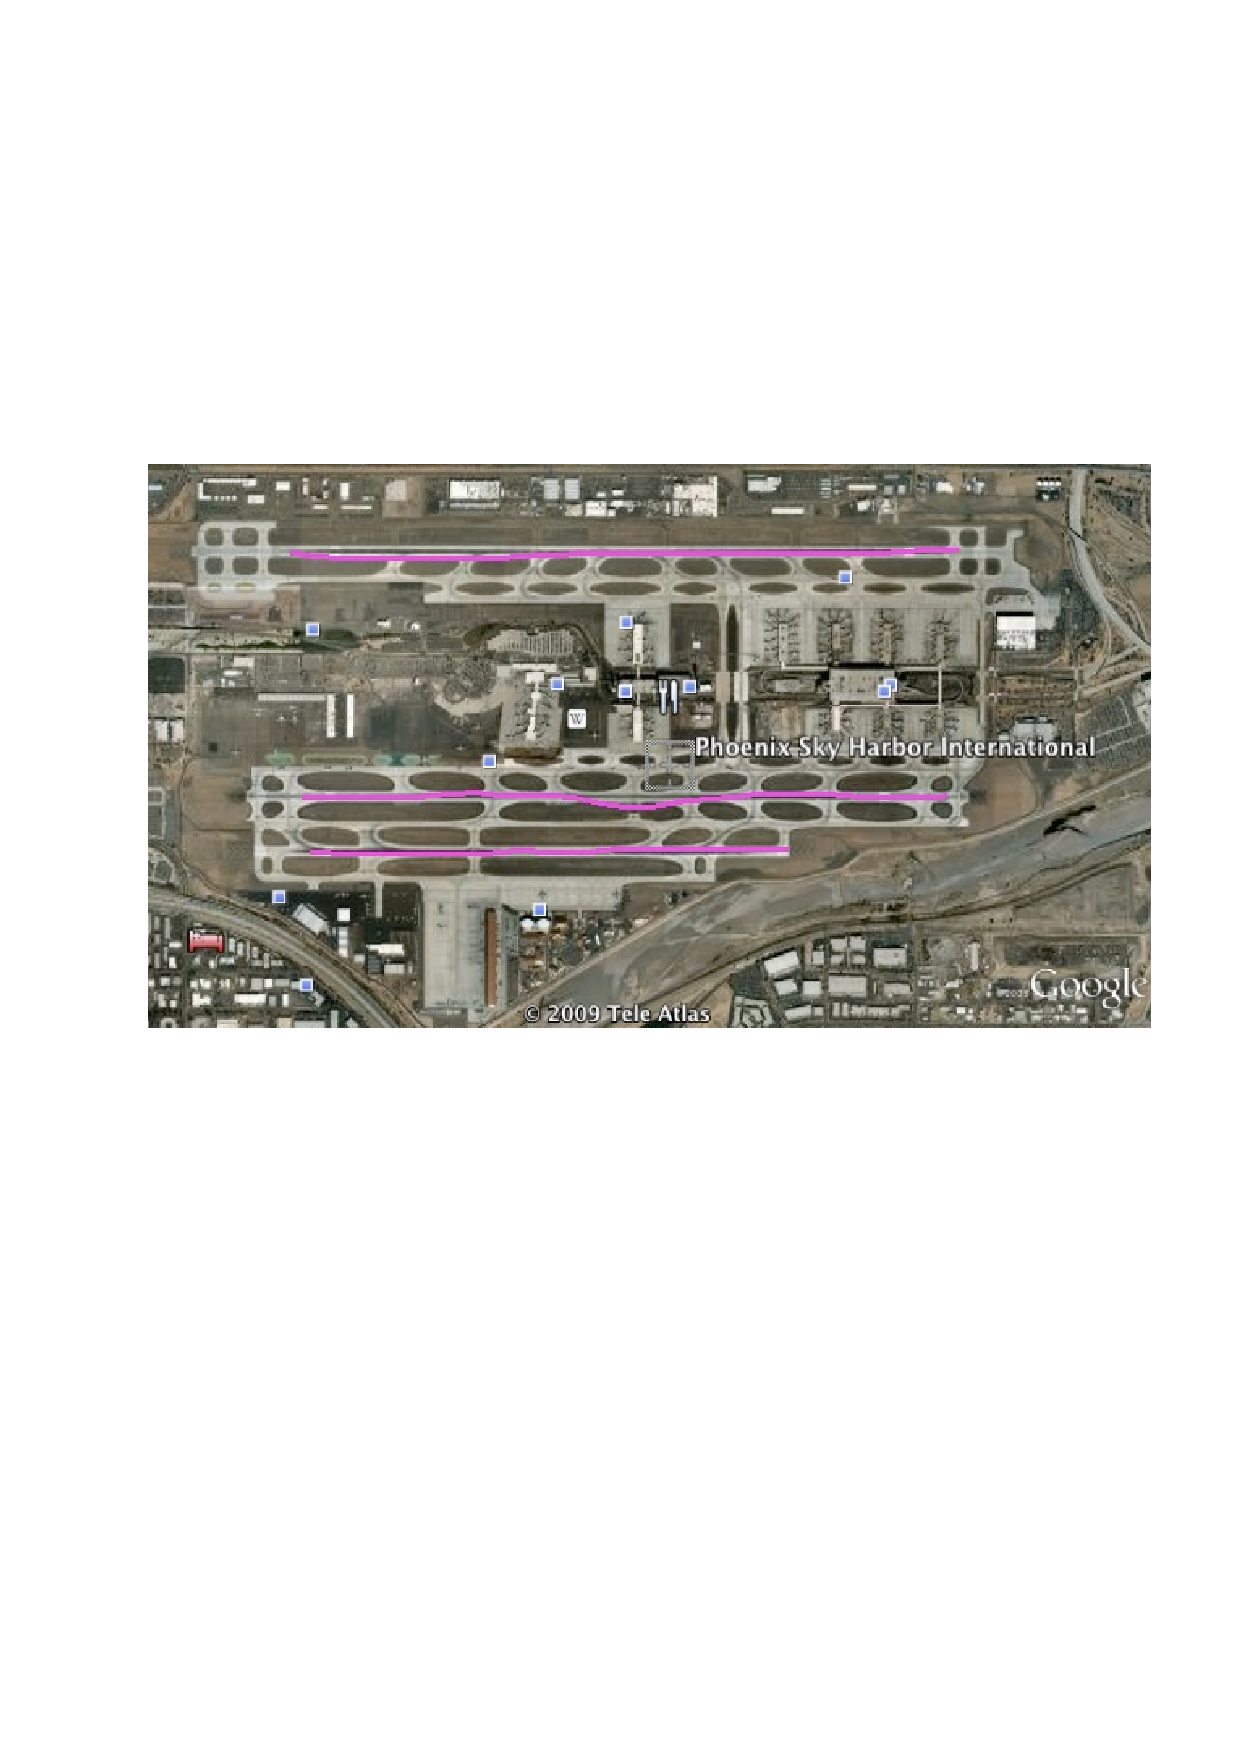
\includegraphics[width=0.35\textwidth]{PHX-airport}
  \end{center}
\vspace{-20pt}
   \caption{\it Phoenix International Airport: all three runways (marked by horizontal lines) are in West-East Direction.}
\vspace{-10pt}
   \label{phx}
\end{wrapfigure}

Figure \ref{phx-test} shows arrival delays plotted against permutations  of wind direction (null plots) as suggested by \cite{buja:2009}. 
%
One plot is of the real data of the observed wind directions. If we can differentiate this plot from  the null plots, we can reject the null hypothesis of crosswinds being unrelated to arrival delays with a $p$-value of less than 1/10 = 0.10. The plot of the data is number four. It is left to the reader to decide, whether this plot is different from the others -- but evidence gathered informally suggests this to be the case (8 out of 10 group members decided on plot number four -- all giving the box in SW as the reason, yielding a theoretical $p$-value of  well below 0.0001)

\begin{figure}[htbp] %  figure placement: here, top, bottom, or page
   \centering
   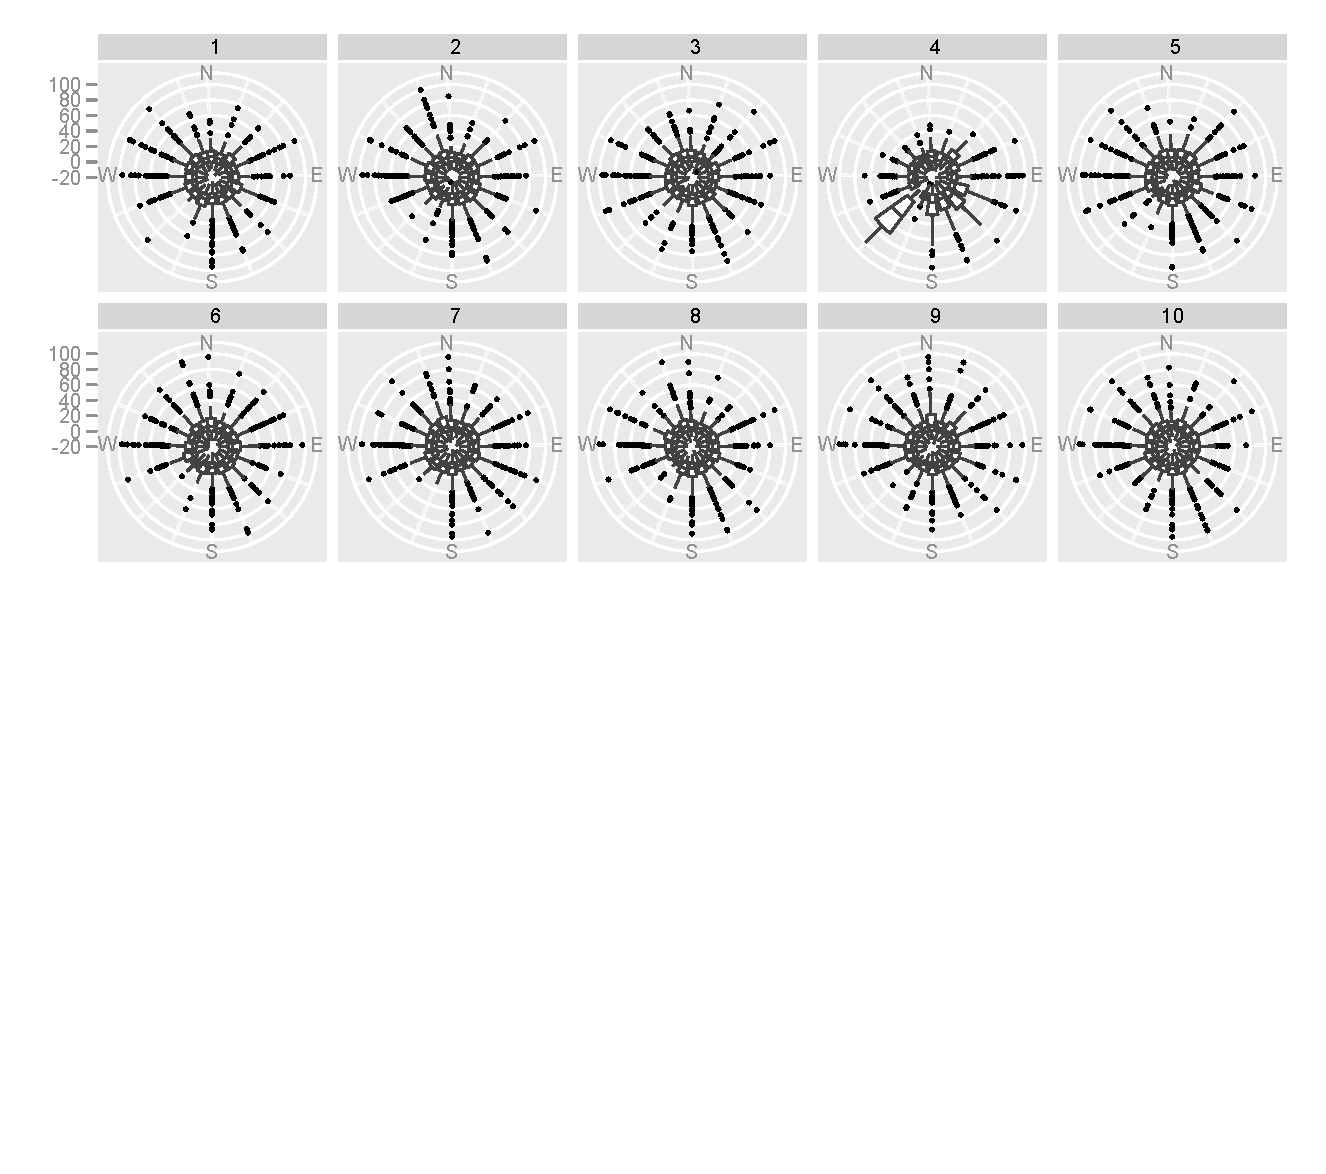
\includegraphics[width=6in]{winds-phoenix} 
\vspace{-10pt}
   \caption{\it Delays (in minutes) by wind direction. Only one plot shows the observed data, the others are permutations (null plots).}
   \label{phx-test}
\end{figure}

\end{document}  